%!TEX root = ../dissertation.tex
\chapter{Introduction}
\label{introduction}

We are currently experiencing a mass extinction event that parallels
other episodes in earth's history with high rates of biodiversity
decline \citep{Pimm1995, Dirzo2003, Schipper2008, Barnosky2011,
Dirzo2014}. Other than the five extinction events preceding it
\citep{Kolbert2014}, it is anthropogenic in origin \citep{Leakey1996,
Ceballos2015} and is associated with global warming \citep{Cook2016,
Wuebbles2017}, large-scale deforestation \citep{Wright2005}, destruction
of marine and freshwater habitats \citep{Burkhead2012}, and introduction
of invasive species \citep{Mooney2001}, all hallmarks of human
influence. Put shortly, the rate at which species go extinct is alarming
\citep{Newbold2016, Ceballos2017, Hallmann2017}, and our children will
likely experience a world with less than half the biodiversity we know
today. While this issue has raised the attention of country leaders and
conservation policies are being put in place worldwide
\citep{Puntaru2017}, this might not be enough to reverse the trend
without sustaining irreparable damage to the ecosystems of the planet.
To make matters worse, there are signs that the issue, despite its
urgency, is fading from public awareness \citep{Kusmanoff2017}. 

Conservation efforts require intimate knowledge of the systems they aim
to preserve: Of course, we cannot save what we do not know. The road
towards understanding the biology and the interaction of species is,
however, traveled on multiple levels. It is not enough to observe the
behaviour or the feeding preferences of an animal to understand the
impact of it being removed from its habitat. It is also not enough to
describe functional morphology to gain insight on ecological
implications. Neither is it sufficient to analyse the genes and draw
conclusions based on their composition and structure. Profound
understanding of any system can only be gained by studying it from
multiple angles and with interdisciplinary approaches. One such approach
is to sequence and analyse the genome of a species: the source code of
life that defines, by a manifold of means, its appearance, features,
behaviour and interactions with the environment.

The genome, that is, the entirety of DNA of an organism is a composition
of different functional complexes. It does not only contain genes, which
are translated into the proteins that make up cells and, ultimately, all
organisms; in fact, the human gene repertoire of around 23,000 genes
makes up only around 2 \% of the human genome \citep{Makalowski2001}
(Figure \ref{fig:human-genome}). More prominent components of the human
genome include introns (non-coding sections of genes, \~26 \%), but by
far the most voluminous chunk consists of repetitive elements: DNA
segments that occur in sometimes many copies throughout the genome.
More than half of the three billion base pairs (Gbp) of the human genome
(52 \%) is occupied by repetitive elements \citep{Lander2001}. The major
part of these repetitive elements in the human genome, also called
repeats, is formed by transposable elements (45 \% of the genome).

\begin{figure}
\centering
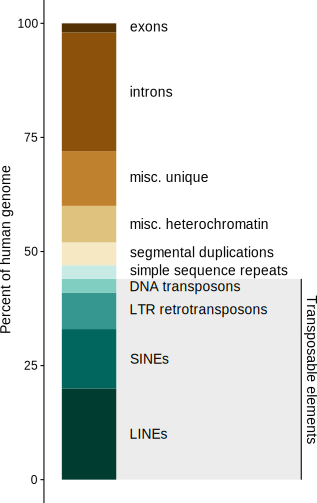
\includegraphics[width=0.3\textwidth]{human}
\caption{Composition of the human genome. Almost half of the three
billion base pairs in the genome is attributed to transposable elements
of various classes.}
\label{fig:human-genome}
\end{figure}

Transposable elements (TEs) are also known as ``jumping genes'' or
``parasitic DNA''. They were discovered in the 1940s by their defining
property, the capability of movement within the genome
\citep{McClintock1950}. By duplicating themselves through various
mechanisms that depend on the TE type, TEs can reach copy numbers in the
thousands \citep{Petersen2018} and, like in the human genome (Figure
\ref{fig:human-genome}), be a major contributor to the genome size. This
genome ``inflation'' effect due to TE proliferation has been observed
throughout eukaryotes in general \citep{Chenais2012}, and reiterated in
vertebrates \citep{Chalopin2015}, arthropods \citep{Petersen2018}, and
plants \citep{Staton2015}. 

The genomes of mammals, such as human, and birds exhibit much less
variation in size than, for example, the genomes of arthropods or even
amphibians \citep{Gregory2005}. In mammals, genome size varies around
five-fold and in birds even only around two-fold, whereas in insects,
the spread is around 240-fold (Table \ref{tab:genome-size-spread} on page
\pageref{tab:genome-size-spread}). This immense variation surpasses that
of amphibians, where some species have huge genomes of up to 118 Gbp, and
is paralleled only by the group of bony fishes (Osteichthyes), which
exhibit a genome size spread of around 390-fold. Before the discovery of
TEs and non-coding DNA in the genome, it was assumed that genome size
should correlate with perceived organismic complexity, but the fact that
amoeba have genomes with up to a staggering 670 Gbp \citep{Parfrey2008}
did not fit well with that assumption. This apparent contradiction was
named the ``C-value paradox'' and later renamed to ``C-value enigma''
\citep{Gregory2007}, as still a connection between genome size and
organismic complexity appears absent.

The genome needs to be maintained: repair mechanisms and transcription
machinery as well as error correction use energy. The error rate
increases with genome size \citep{Wielgoss2011}, making more repairs
necessary. Larger genome size has been linked to decreased development
rate \citep{White2000} and increased oxygen requirements
\citep{Vinogradov1997, Gregory2002}. In plants \citep{Grime1983},
invertebrates \citep{Gregory2005}, and vertebrates \citep{Horner1983,
Olmo1982, Gregory2000}, it has been shown that cell size increases with
genome size \citep{Dufresne2011}. Larger cells are also costly to
maintain and proliferate, and they divide more slowly
\citep{Bennett1977}. In summary, a large genome comes with a cost.


\begin{table}[h]
\centering
\caption{Genome size spread in Eukaryotes. Values are in picogram DNA;
one pg is approx. 978 mega-basepairs (Mbp). Data from the Genome Size
Database \citep{Gregory2018}, \url{http://www.genomesize.com}, accessed
2018-05-07.}
\label{tab:genome-size-spread}
\begin{tabular}{@{}llrrr@{}}
\toprule
Subphylum  & Class              & Min  & Max    & $\Delta$fold  \\
\midrule
Crustacea  & Branchiopoda       & 0.16 &   2.91 &  18.19        \\
Crustacea  & Copepoda           & 0.14 &  14.68 & 104.86        \\
Crustacea  & Malacostraca       & 0.68 &  64.62 &  95.03        \\
Crustacea  & Ostracoda          & 0.46 &   3.13 &   6.80        \\
Hexapoda   & Insecta            & 0.07 &  16.93 & 241.86        \\
Vertebrata & Amphibia           & 0.95 & 120.60 & 126.95        \\
Vertebrata & Aves               & 0.91 &   2.16 &   2.37        \\
Vertebrata & Chondrichthyes     & 1.51 &  17.05 &  11.29        \\
Vertebrata & Mammalia           & 1.63 &   8.40 &   5.15        \\
Vertebrata & Osteichthyes       & 0.34 & 132.83 & 390.68        \\
Vertebrata & Reptilia           & 1.05 &   5.44 &   5.18        \\
\bottomrule
\end{tabular}
\end{table}


